\documentclass[aspectratio=169]{beamer}
\usetheme{Madrid}
\usecolortheme{default}

% Packages
\usepackage{graphicx}
\usepackage{tikz}
\usepackage{amsmath}
\usepackage{xcolor}
\usepackage{listings}

% Title page information
\title{Automated Star Identification System}
\subtitle{From Image Input to Labeled Star Map}
\author{Your Name}
\institute{Your Institution}
\date{\today}

% Define custom colors
\definecolor{starblue}{RGB}{30,144,255}
\definecolor{starred}{RGB}{220,20,60}
\definecolor{stargreen}{RGB}{34,139,34}

\begin{document}

% Title slide
\frame{\titlepage}

% Outline
\begin{frame}{Presentation Outline}
\tableofcontents
\end{frame}

\section{Introduction}

\begin{frame}{What Does This System Do?}
\begin{center}
\Large
\textbf{Input:} A photo of the night sky \\[0.5cm]
\textbf{Output:} The same photo with stars labeled by name \\[1cm]

\textcolor{starblue}{\textbf{Think of it as "Shazam for Stars"}}
\end{center}

\begin{itemize}
\item Take any astronomical image
\item Automatically identify which stars are visible
\item Label them with proper names and information
\item No manual star charts needed!
\end{itemize}
\end{frame}

\begin{frame}{Why Is This Challenging?}
\begin{columns}
\begin{column}{0.5\textwidth}
\textbf{Human Challenges:}
\begin{itemize}
\item Thousands of stars visible
\item Stars look very similar
\item Need extensive astronomy knowledge
\item Time-consuming process
\end{itemize}
\end{column}

\begin{column}{0.5\textwidth}
\textbf{Computer Challenges:}
\begin{itemize}
\item Distinguish stars from noise
\item Determine viewing direction
\item Match patterns to database
\item Handle image variations
\end{itemize}
\end{column}
\end{columns}

\vspace{0.5cm}
\begin{center}
\textcolor{starred}{\textbf{Solution: Break into 6 manageable steps!}}
\end{center}
\end{frame}

\section{Algorithm Overview}

\begin{frame}{The 6-Step Algorithm Pipeline}
\begin{center}
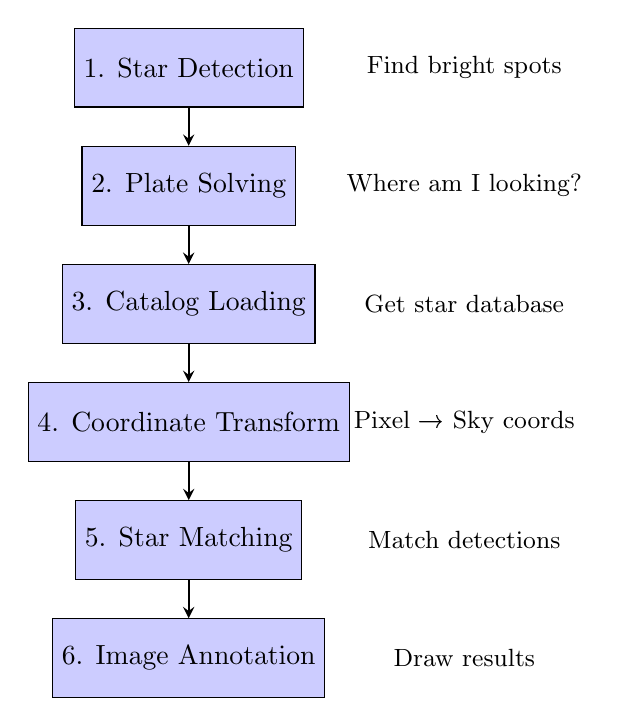
\begin{tikzpicture}[node distance=1.5cm, auto]
% Define styles
\tikzstyle{process} = [rectangle, minimum width=2.5cm, minimum height=1cm, text centered, draw=black, fill=blue!20]
\tikzstyle{arrow} = [thick,->,>=stealth]

% Draw nodes
\node [process] (step1) {1. Star Detection};
\node [process, below of=step1] (step2) {2. Plate Solving};
\node [process, below of=step2] (step3) {3. Catalog Loading};
\node [process, below of=step3] (step4) {4. Coordinate Transform};
\node [process, below of=step4] (step5) {5. Star Matching};
\node [process, below of=step5] (step6) {6. Image Annotation};

% Draw arrows
\draw [arrow] (step1) -- (step2);
\draw [arrow] (step2) -- (step3);
\draw [arrow] (step3) -- (step4);
\draw [arrow] (step4) -- (step5);
\draw [arrow] (step5) -- (step6);

% Add side labels
\node [right of=step1, node distance=3.5cm] {\small Find bright spots};
\node [right of=step2, node distance=3.5cm] {\small Where am I looking?};
\node [right of=step3, node distance=3.5cm] {\small Get star database};
\node [right of=step4, node distance=3.5cm] {\small Pixel → Sky coords};
\node [right of=step5, node distance=3.5cm] {\small Match detections};
\node [right of=step6, node distance=3.5cm] {\small Draw results};
\end{tikzpicture}
\end{center}
\end{frame}

\section{Step 1: Star Detection}

\begin{frame}{Step 1: Star Detection}
\begin{columns}
\begin{column}{0.6\textwidth}
\textbf{Goal:} Find all bright objects that could be stars

\textbf{Algorithm Steps:}
\begin{enumerate}
\item Convert photo to grayscale
\item Apply Gaussian blur (reduce noise)
\item Binary thresholding (bright vs dark)
\item Find contours (connected bright regions)
\item Filter by size (remove noise \& artifacts)
\end{enumerate}

\textbf{Real-world analogy:}
\textcolor{starblue}{Like using a highlighter to mark all bright spots on a printed photo}
\end{column}

\begin{column}{0.4\textwidth}
\begin{center}
\textbf{Visual Process:}
\\[0.3cm]
Original Image \\
↓ \\
Grayscale \\
↓ \\
Blur \\
↓ \\
Threshold \\
↓ \\
\textcolor{starred}{Detected Stars}
\end{center}
\end{column}
\end{columns}

\vspace{0.5cm}
\textbf{Output:} List of (x,y) coordinates where stars are detected
\end{frame}

\begin{frame}{Star Detection: Key Parameters}
\begin{itemize}
\item \textbf{Threshold Value (120):} How bright must a spot be?
\begin{itemize}
\item Lower → detect fainter stars (more noise)
\item Higher → only brightest stars (miss faint ones)
\end{itemize}

\item \textbf{Minimum Area (1 pixel):} Smallest acceptable star
\begin{itemize}
\item Filters out single-pixel noise
\end{itemize}

\item \textbf{Maximum Area (800 pixels):} Largest acceptable star
\begin{itemize}
\item Removes planets, satellites, defects
\end{itemize}

\item \textbf{Gaussian Blur (3×3):} Noise reduction
\begin{itemize}
\item Smooths image while preserving star shapes
\end{itemize}
\end{itemize}

\textcolor{stargreen}{\textbf{Typical Result:} 20-100 detected bright spots per image}
\end{frame}

\section{Step 2: Plate Solving}

\begin{frame}{Step 2: Plate Solving (Astrometric Calibration)}
\textbf{Goal:} Determine which part of the sky we're looking at

\begin{columns}
\begin{column}{0.5\textwidth}
\textbf{Method 1 - Astrometry.net API:}
\begin{enumerate}
\item Upload image to online service
\item Service compares star patterns
\item Returns sky coordinates \& field of view
\item Like fingerprint matching!
\end{enumerate}

\textcolor{stargreen}{Most accurate method}
\end{column}

\begin{column}{0.5\textwidth}
\textbf{Method 2 - Filename Patterns:}
\begin{enumerate}
\item Check filename for keywords
\item "orion.jpg" → Orion coordinates
\item "m42\_nebula.png" → M42 coordinates  
\item Use pre-programmed locations
\end{enumerate}

\textcolor{starred}{Fallback when API fails}
\end{column}
\end{columns}

\vspace{0.5cm}
\textbf{Real-world analogy:} \textcolor{starblue}{Like using GPS to find your location, but for space photos}

\vspace{0.3cm}
\textbf{Output:} Image center coordinates (RA, Dec) and field of view radius
\end{frame}

\begin{frame}{Why Plate Solving Is Crucial}
\begin{center}
\textbf{Without knowing WHERE you're looking...}
\\[0.5cm]
You can't match detected spots to known stars!
\end{center}

\vspace{0.5cm}
\textbf{What we get:}
\begin{itemize}
\item \textbf{RA (Right Ascension):} Like longitude for space (0-360°)
\item \textbf{Dec (Declination):} Like latitude for space (-90° to +90°)  
\item \textbf{Field of View:} How much sky the image covers
\end{itemize}

\vspace{0.5cm}
\textbf{Example Results:}
\begin{itemize}
\item Orion constellation: RA = 85°, Dec = -1°, FOV = 15°
\item Pleiades cluster: RA = 57°, Dec = 24°, FOV = 5°
\end{itemize}
\end{frame}

\section{Step 3: Catalog Loading}

\begin{frame}{Step 3: Star Catalog Loading}
\textbf{Goal:} Get list of known stars that should be visible in our image

\begin{columns}
\begin{column}{0.6\textwidth}
\textbf{The Database:} Yale Bright Star Catalog v5
\begin{itemize}
\item Contains 9,000 brightest stars
\item For each star: name, position, brightness, spectral type
\item Covers entire sky down to magnitude ~6.5
\end{itemize}

\textbf{Search Process:}
\begin{enumerate}
\item "Give me all stars within 15° of (85°, -1°)"
\item Database returns ~100-500 stars in region
\item Sort by brightness (magnitude)
\end{enumerate}
\end{column}

\begin{column}{0.4\textwidth}
\begin{center}
\textbf{Sample Star Data:}
\\[0.3cm]
\begin{tabular}{|l|c|}
\hline
\textbf{Name} & \textbf{Sirius} \\
\hline
HR Number & 2491 \\
\hline
RA & 101.29° \\
\hline
Dec & -16.72° \\
\hline
Magnitude & -1.46 \\
\hline
Type & A1V \\
\hline
\end{tabular}
\end{center}
\end{column}
\end{columns}

\vspace{0.5cm}
\textbf{Real-world analogy:} \textcolor{starblue}{Like opening a phone book for your neighborhood}
\end{frame}

\section{Step 4: Coordinate Transformation}

\begin{frame}{Step 4: Coordinate Transformation}
\textbf{Goal:} Convert detected pixel positions to sky coordinates

\begin{center}
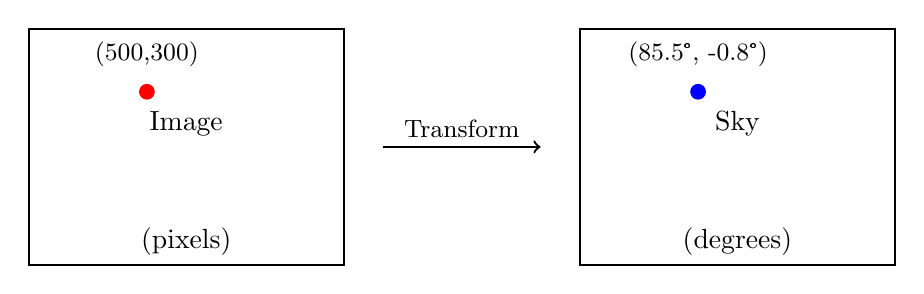
\begin{tikzpicture}
% Draw image representation
\draw[thick] (0,0) rectangle (4,3);
\node at (2,1.8) {Image};
\node at (2,0.3) {(pixels)};

% Draw detected star
\fill[red] (1.5,2.2) circle (0.1);
\node[above] at (1.5,2.4) {\small (500,300)};

% Arrow
\draw[thick,->] (4.5,1.5) -- (6.5,1.5);
\node[above] at (5.5,1.5) {\small Transform};

% Draw sky representation  
\draw[thick] (7,0) rectangle (11,3);
\node at (9,1.8) {Sky};
\node at (9,0.3) {(degrees)};

% Draw transformed star
\fill[blue] (8.5,2.2) circle (0.1);
\node[above] at (8.5,2.4) {\small (85.5°, -0.8°)};
\end{tikzpicture}
\end{center}

\textbf{Mathematical Process:}
\begin{enumerate}
\item Calculate pixel scale: $\frac{\text{field of view}}{\text{image size}}$ degrees/pixel
\item Find offset from image center
\item Convert pixel offset to angular offset  
\item Apply spherical coordinate correction
\item Add to image center coordinates
\end{enumerate}

\textbf{Real-world analogy:} \textcolor{starblue}{Like converting "3 inches right on map" to "50 miles east in reality"}
\end{frame}

\begin{frame}{Coordinate Transformation: The Math}
\textbf{Key Equations:}

\begin{align}
\text{Pixel Scale} &= \frac{\text{Field of View} \times 2}{\min(\text{width}, \text{height})} \text{ deg/pixel} \\[0.3cm]
\text{Angular Offset}_x &= (\text{pixel}_x - \text{center}_x) \times \text{Pixel Scale} \\[0.3cm]
\text{Angular Offset}_y &= -(\text{pixel}_y - \text{center}_y) \times \text{Pixel Scale} \\[0.3cm]
\text{Star RA} &= \text{Image RA} + \frac{\text{Angular Offset}_x}{\cos(\text{Dec})} \\[0.3cm]
\text{Star Dec} &= \text{Image Dec} + \text{Angular Offset}_y
\end{align}

\vspace{0.3cm}
\textbf{Important Notes:}
\begin{itemize}
\item Y-axis is flipped (image vs sky coordinates)
\item RA correction needed for spherical geometry
\item Simple linear projection (good for small fields)
\end{itemize}
\end{frame}

\begin{frame}{Coordinate Transformation: Example}
\textbf{Given:} Orion image, 1000×800 pixels, FOV = 15°, center at RA=85°, Dec=-1°

\textbf{Step 1: Calculate pixel scale}
\begin{align}
\text{Pixel Scale} &= \frac{15° \times 2}{\min(1000, 800)} = \frac{30°}{800} = 0.0375 \text{ deg/pixel}
\end{align}

\textbf{Step 2: Find a detected star at pixel (650, 300)}
\begin{align}
\text{Angular Offset}_x &= (650 - 500) \times 0.0375 = 150 \times 0.0375 = 5.625° \\
\text{Angular Offset}_y &= -(300 - 400) \times 0.0375 = -(-100) \times 0.0375 = 3.75°
\end{align}

\textbf{Step 3: Convert to sky coordinates}
\begin{align}
\text{Star RA} &= 85° + \frac{5.625°}{\cos(-1°)} = 85° + 5.628° = 90.628° \\
\text{Star Dec} &= -1° + 3.75° = 2.75°
\end{align}

\textcolor{stargreen}{\textbf{Result:} Pixel (650,300) → Sky coordinates (90.63°, 2.75°)}

\textcolor{starblue}{\textbf{This could be Betelgeuse at RA=88.8°, Dec=7.4°!}}
\end{frame}

\section{Algorithm Evolution}

\begin{frame}{Algorithm Evolution: Part 1 vs Part 2}
\begin{columns}
\begin{column}{0.5\textwidth}
\textbf{Part 1: Geometric Pattern Matching}
\begin{itemize}
\item Used \textcolor{starred}{triangle} and \textcolor{starred}{quadrilateral} patterns
\item Matched star \textcolor{starred}{shapes} between images
\item Calculated normalized side lengths
\item Robust to rotation and scaling
\item Complex voting system
\end{itemize}

\textbf{Advantages:}
\begin{itemize}
\item Works without sky coordinates
\item Handles image transformations
\item More sophisticated matching
\end{itemize}
\end{column}

\begin{column}{0.5\textwidth}
\textbf{Part 2: Coordinate-Based Matching}
\begin{itemize}
\item Uses \textcolor{stargreen}{sky coordinates} (RA/Dec)
\item Matches by \textcolor{stargreen}{angular distance}
\item Simple nearest-neighbor algorithm
\item Relies on plate solving
\item Direct star-to-catalog matching
\end{itemize}

\textbf{Advantages:}
\begin{itemize}
\item Much faster processing
\item Simpler to understand
\item Works with star catalogs
\item Real astronomical coordinates
\end{itemize}
\end{column}
\end{columns}

\vspace{0.5cm}
\begin{center}
\textcolor{starblue}{\textbf{Evolution: From image-to-image matching → image-to-catalog matching}}
\end{center}
\end{frame}

\begin{frame}{Triangle Algorithm (Part 1) - How It Worked}
\textbf{Geometric Pattern Matching Process:}

\begin{enumerate}
\item \textbf{Find Neighbors:} For each star, find k=5 nearest neighbors
\item \textbf{Form Triangles:} Create triangles from star + 2 neighbors
\item \textbf{Calculate Distances:} Measure all 3 side lengths
\item \textbf{Normalize:} Divide by longest side → pattern ratios
\item \textbf{Match Patterns:} Compare triangle ratios between images
\item \textbf{Vote:} Triangles vote for star correspondences
\end{enumerate}

\begin{center}
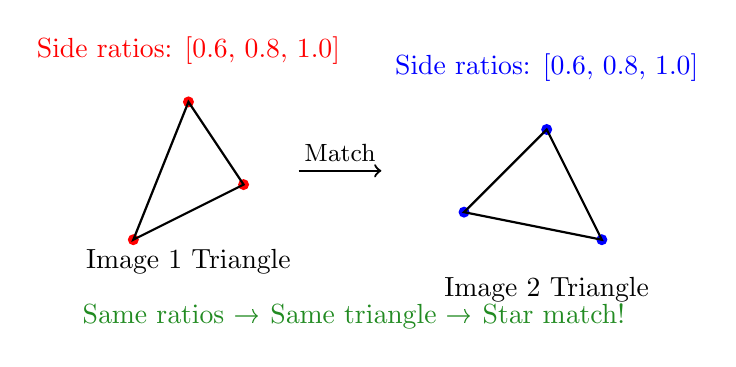
\begin{tikzpicture}[scale=0.7]
% Draw first triangle
\fill[red] (0,0) circle (0.1);
\fill[red] (2,1) circle (0.1);
\fill[red] (1,2.5) circle (0.1);
\draw[thick] (0,0) -- (2,1) -- (1,2.5) -- cycle;
\node[below] at (1,0) {Image 1 Triangle};

% Arrow
\draw[thick,->] (3,1.25) -- (4.5,1.25);
\node[above] at (3.75,1.25) {\small Match};

% Draw second triangle (scaled/rotated)
\fill[blue] (6,0.5) circle (0.1);
\fill[blue] (7.5,2) circle (0.1);
\fill[blue] (8.5,0) circle (0.1);
\draw[thick] (6,0.5) -- (7.5,2) -- (8.5,0) -- cycle;
\node[below] at (7.5,-0.5) {Image 2 Triangle};

% Labels
\node[above] at (1,3) {\textcolor{red}{Side ratios: [0.6, 0.8, 1.0]}};
\node[above] at (7.5,2.7) {\textcolor{blue}{Side ratios: [0.6, 0.8, 1.0]}};
\node[below] at (4,-1) {\textcolor{stargreen}{Same ratios → Same triangle → Star match!}};
\end{tikzpicture}
\end{center}
\end{frame}

\begin{frame}{Why We Changed Approaches}
\textbf{Challenges with Triangle Matching:}
\begin{itemize}
\item \textcolor{starred}{Computationally expensive:} O(n³) complexity for triangles
\item \textcolor{starred}{Image-to-image only:} Couldn't match to star catalogs
\item \textcolor{starred}{Complex voting:} Multiple algorithms, harder to debug
\item \textcolor{starred}{No real star names:} Just matched pixel patterns
\end{itemize}

\textbf{Benefits of Coordinate Matching:}
\begin{itemize}
\item \textcolor{stargreen}{Real astronomy:} Uses actual sky coordinates
\item \textcolor{stargreen}{Star identification:} Get real star names and data
\item \textcolor{stargreen}{Faster:} O(m×n) where m,n are much smaller
\item \textcolor{stargreen}{Simpler:} Easier to understand and modify
\item \textcolor{stargreen}{Catalog integration:} Works with professional databases
\end{itemize}

\vspace{0.5cm}
\begin{center}
\textbf{Trade-off:} Sacrificed geometric robustness for astronomical accuracy
\end{center}
\end{frame}

\section{Step 5: Star Matching}

\begin{frame}{Step 5: Star Matching Algorithm (Current Approach)}
\textbf{Goal:} Match detected bright spots with known catalog stars

\textbf{Algorithm: Greedy Nearest-Neighbor}
\begin{enumerate}
\item Take brightest catalog star
\item Find closest detected spot within 0.8°
\item If match found, pair them up
\item Remove both from available pools
\item Repeat with next brightest catalog star
\end{enumerate}

\begin{center}
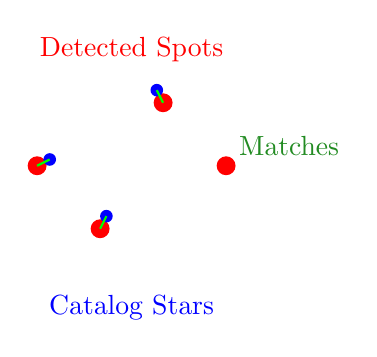
\begin{tikzpicture}[scale=0.8]
% Draw detected stars
\fill[red] (1,2) circle (0.15);
\fill[red] (3,3) circle (0.15);
\fill[red] (2,1) circle (0.15);
\fill[red] (4,2) circle (0.15);
\node[above] at (2.5,3.5) {\textcolor{red}{Detected Spots}};

% Draw catalog stars
\fill[blue] (1.2,2.1) circle (0.1);
\fill[blue] (2.9,3.2) circle (0.1);
\fill[blue] (2.1,1.2) circle (0.1);
\node[below] at (2.5,0.1) {\textcolor{blue}{Catalog Stars}};

% Draw matching lines
\draw[green, thick] (1,2) -- (1.2,2.1);
\draw[green, thick] (3,3) -- (2.9,3.2);
\draw[green, thick] (2,1) -- (2.1,1.2);

% Label
\node[above] at (5,2) {\textcolor{stargreen}{Matches}};
\end{tikzpicture}
\end{center}

\textbf{Real-world analogy:} \textcolor{starblue}{Like matching faces in a group photo to a class roster}
\end{frame}

\begin{frame}{Star Matching: Key Considerations}
\textbf{Why 0.8° threshold?}
\begin{itemize}
\item Accounts for measurement errors
\item Coordinate conversion uncertainties  
\item Star catalog precision limits
\item Atmospheric effects
\end{itemize}

\textbf{Why brightest stars first?}
\begin{itemize}
\item More likely to be correctly detected
\item Higher confidence matches
\item Reduces false positives
\end{itemize}

\textbf{One-to-one matching:}
\begin{itemize}
\item Each detected spot matched to at most one catalog star
\item Prevents duplicate assignments
\item Ensures unique identifications
\end{itemize}

\textcolor{stargreen}{\textbf{Typical Result:} 5-25 successful matches per image (10-20\% success rate)}
\end{frame}

\section{Step 6: Image Annotation}

\begin{frame}{Step 6: Image Annotation}
\textbf{Goal:} Create beautiful labeled star map

\begin{columns}
\begin{column}{0.5\textwidth}
\textbf{Visual Elements:}
\begin{itemize}
\item \textcolor{starred}{\textbf{Red circles:}} All detected spots
\item \textcolor{stargreen}{\textbf{Green circles:}} Identified stars  
\item \textbf{Yellow labels:} Star names \& info
\item \textbf{Arrows:} Connect labels to stars
\item \textbf{Title:} Summary statistics
\end{itemize}

\textbf{Information Displayed:}
\begin{itemize}
\item Star name (e.g., "Sirius")
\item Harvard Revised number (HR2491)
\item Visual magnitude (-1.46)
\item Total detection/identification counts
\end{itemize}
\end{column}

\begin{column}{0.5\textwidth}
\begin{center}
\textbf{Sample Output:}
\\[0.5cm]
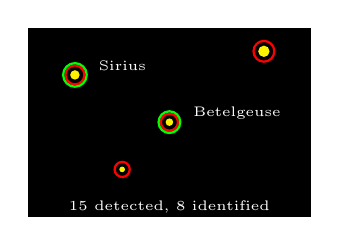
\begin{tikzpicture}[scale=0.6]
% Background
\fill[black] (0,0) rectangle (6,4);

% Stars
\fill[yellow] (1,3) circle (0.1);
\fill[yellow] (3,2) circle (0.08);
\fill[yellow] (5,3.5) circle (0.12);
\fill[yellow] (2,1) circle (0.06);

% Red circles (detected)
\draw[red, thick] (1,3) circle (0.2);
\draw[red, thick] (3,2) circle (0.18);
\draw[red, thick] (5,3.5) circle (0.22);
\draw[red, thick] (2,1) circle (0.16);

% Green circles (identified)  
\draw[green, thick] (1,3) circle (0.25);
\draw[green, thick] (3,2) circle (0.23);

% Labels
\node[white, right] at (1.3,3.2) {\tiny Sirius};
\node[white, right] at (3.3,2.2) {\tiny Betelgeuse};

% Title
\node[white] at (3,0.2) {\tiny 15 detected, 8 identified};
\end{tikzpicture}
\end{center}
\end{column}
\end{columns}

\textbf{Real-world analogy:} \textcolor{starblue}{Like adding captions to a photo}
\end{frame}

\section{System Performance}

\begin{frame}{System Performance \& Results}
\begin{columns}
\begin{column}{0.5\textwidth}
\textbf{Typical Performance:}
\begin{itemize}
\item \textbf{Input:} 50-100 visible stars
\item \textbf{Detected:} 20-80 bright spots  
\item \textbf{Identified:} 5-25 named stars
\item \textbf{Success Rate:} 10-20\%
\item \textbf{Processing Time:} 5-30 seconds
\end{itemize}

\textbf{Best Results With:}
\begin{itemize}
\item Clear, focused star images
\item 5-20° field of view
\item Bright stars (magnitude < 4)
\item Good contrast photos
\end{itemize}
\end{column}

\begin{column}{0.5\textwidth}
\textbf{Limitations:}
\begin{itemize}
\item Only 9,000 brightest stars in catalog
\item Requires internet for best plate solving
\item Struggles with very wide/narrow fields
\item Can't identify faint deep-sky objects
\end{itemize}

\textbf{Common Issues:}
\begin{itemize}
\item Overexposed images
\item Out-of-focus stars
\item Light pollution
\item Clouds or atmospheric haze
\end{itemize}
\end{column}
\end{columns}

\vspace{0.5cm}
\textcolor{stargreen}{\textbf{Overall: Excellent tool for amateur astronomy and education!}}
\end{frame}

\section{Applications}

\begin{frame}{Real-World Applications}
\begin{columns}
\begin{column}{0.5\textwidth}
\textbf{Educational:}
\begin{itemize}
\item Astronomy classes
\item Planetarium shows  
\item Student projects
\item Public outreach
\end{itemize}

\textbf{Amateur Astronomy:}
\begin{itemize}
\item Astrophotography labeling
\item Observation planning
\item Star party activities
\item Equipment testing
\end{itemize}
\end{column}

\begin{column}{0.5\textwidth}
\textbf{Professional:}
\begin{itemize}
\item Telescope automation
\item Camera calibration
\item Archive processing
\item Research applications
\end{itemize}

\textbf{Fun Applications:}
\begin{itemize}
\item Social media posts
\item Travel photography
\item Citizen science
\item Mobile apps
\end{itemize}
\end{column}
\end{columns}

\vspace{0.5cm}
\begin{center}
\textcolor{starblue}{\textbf{Making astronomy accessible to everyone!}}
\end{center}
\end{frame}

\section{Technical Implementation}

\begin{frame}{Technical Architecture}
\textbf{System Components:}

\begin{itemize}
\item \textbf{star\_algorithm.py:} Core algorithmic logic
\begin{itemize}
\item All 6 algorithm steps implemented here
\item Pure computational functions
\item No web interface dependencies
\end{itemize}

\item \textbf{flask\_star\_identifier.py:} Web server wrapper  
\begin{itemize}
\item HTTP endpoints for image upload
\item File handling and validation
\item JSON result formatting
\item User interface integration
\end{itemize}
\end{itemize}

\textbf{Key Technologies:}
\begin{itemize}
\item \textbf{OpenCV:} Computer vision and image processing
\item \textbf{NumPy/Pandas:} Numerical computations and data handling
\item \textbf{SQLite:} Star catalog database
\item \textbf{Flask:} Web framework for user interface
\item \textbf{Astrometry.net:} Professional plate solving service
\end{itemize}
\end{frame}

\section{Conclusion}

\begin{frame}{Key Takeaways}
\textbf{What We Accomplished:}
\begin{itemize}
\item Automated star identification from photos
\item Robust 6-step algorithmic pipeline
\item Web-based user interface
\item Real-world practical applications
\end{itemize}

\textbf{Algorithm Strengths:}
\begin{itemize}
\item \textcolor{stargreen}{Combines multiple approaches} (CV + databases + web APIs)
\item \textcolor{stargreen}{Handles real-world challenges} (noise, errors, failures)
\item \textcolor{stargreen}{Provides useful results} (10-20\% identification rate)
\item \textcolor{stargreen}{Easy to use} (just upload a photo!)
\end{itemize}

\textbf{Future Improvements:}
\begin{itemize}
\item Larger star catalogs (Gaia, Hipparcos)
\item Better coordinate transformations
\item Machine learning enhancement
\item Mobile app development
\end{itemize}
\end{frame}

\begin{frame}{Questions \& Discussion}
\begin{center}
\Huge Thank You! \\[1cm]

\Large Questions?

\vspace{1cm}

\normalsize
\textcolor{starblue}{\textbf{Demonstration available at:}} \\
Your Flask server URL \\[0.5cm]

\textcolor{stargreen}{\textbf{Code available at:}} \\
Your GitHub repository
\end{center}
\end{frame}

\end{document}